\setcounter{chapter}{-1}
\chapter{Draft to be distilled in 1 and 2}

\minitoc
\newpage

\section{Formal presentation}

In this section, we present notions related to our domains of interest. In particular, for tensors we give original definitions that are more appropriate for our study. In the neural network's section, we present the concepts necessary to understand the evolution of the state of the art research in this field. In the last section, we present graphs for their usage of in deep learning.

Vector spaces considered in what follows are assumed to be finite-dimensional and over the field of real numbers $\bbr$.

\subsection{Tensors}

Intuitively, tensors in the field of deep learning are defined as a generalization of vectors and matrices, as if vectors were tensors of rank $1$ and matrices were tensors of rank $2$. That is, they are objects in a linear space and their dimensions are indexed using as many indices as their rank, so that they can be represented by multidimensional arrays. In mathematics, a tensor is usually defined as a special class of multilinear functions. As such, a mathematical tensor is entirely defined on the cartesian product of the canonical bases onto which its outputs can be represented by a multidimensional array. In that sense, both definitions rejoin on their representation, but the underlying objects are different. In particular, mathematical tensors enjoy a more intrinsic definition as they neither depend on their multidimensional array representation nor on a change of basis.

Our definition of tensors is such that they are a bit more than multidimensional arrays but not as much as mathematical tensors, for that they are embedded in a linear space and any deep learning object can be later define rigorously.

\begin{definition}\textbf{Tensor space}\\
We define a \emph{tensor space} $\bbt$ of rank $r$ as a cartesian product of $r$ vector spaces under the coordinate-wise sum and the mono-linear outer product.

Its \emph{shape} is denoted $n_1 \times n_2 \times \cdots \times n_r$, where the $\{n_k\}$ are the dimensions of the vector spaces.
\end{definition}

Hence, a tensor space is a linear space. Note that for naming conveniency, we distinguish between the terms \emph{linear space} and \emph{vector space}. That is, we abusively use the term \emph{vector space} only to refer to a linear space that can be seen as a tensor space of rank $1$. If there is no notion of rank defined, we rather use the term \emph{linear space}.
We also make a clear distinction between the term \emph{dimension} (that is, for a tensor space it is equal to $\displaystyle \prod_{k=1}^r n_k$) and the term \emph{rank} (equal to $r$).

\begin{definition}\textbf{Tensor}\\
A \emph{tensor} $t$ is an object of a tensor space. The \emph{shape} of $t$, which is the same as the shape of the tensor space it belongs to, is denoted $n_1^{(t)} \times n_2^{(t)} \times \cdots \times n_r^{(t)}$.
\end{definition}

\begin{definition}\textbf{Indexing}\\
An \emph{entry} of a tensor $t$ is a scalar denoted $t[i_1, i_2, \ldots, i_r]$.

A \emph{subtensor} $t'$ is a tensor of same rank composed of entries of $t$ that are contiguous in the indexing, with at least one entry per rank. We denote $t' = t[l_1{:}u_1, l_2{:}u_2, \ldots, l_r{:}u_r]$, where the $\{l_p\}$ and the $\{u_p\}$ are the lower and upper bounds of the indices used by the entries that compose~$t'$.
\end{definition}

When using an index $i_k$ for an entry of a tensor $t$, we implicitly assume that $i_k \in \{1, 2, \cdots, n_k^{(t)}\}$ if nothing is precised.
For subtensor indexings, we don't necessarily write the lower bound index if it is equal to $1$, neither the upper bound index if it is equal to $n_p^{(t)}$.

\begin{definition}\textbf{Slicing}\\
A \emph{slice} operation, along the last ranks $\{r_1, r_2, \ldots, r_s\}$, and indexed by $(i_{r_1}, i_{r_2}, \ldots, i_{r_s})$, is a morphism $s: \bbt = \displaystyle \prod_{k=1}^r \bbv_k \rightarrow \prod_{k=1}^{r-s} \bbv_k$, such that:
\begin{align*}
s(t)[i'_1, i'_2, \ldots, i'_{r-s}] &= t[i'_1, i'_2, \ldots, i'_{r-s}, i_{r_1}, i_{r_2}, \ldots, i_{r_s}] \\
\text{ i.e. } \quad s(t) :&= t[:,:, \ldots, :, i_{r_1}, i_{r_2}, \ldots, i_{r_s}]
\end{align*}
where $:=$ means that values of the right operand are assigned to the left operand.
We denote $t_{i_{r_1}, i_{r_2}, \ldots i_{r_s}}$ and call it the \emph{slice} of $t$. 
Slicing along a subset of ranks that are not the lasts is defined similarly.
$s(\bbt)$ is called a \emph{sliced subspace}.
\end{definition}

\begin{definition}\textbf{Flattening}\\
A \emph{flatten} operation is an isomorphism $f: \bbt \rightarrow \bbv$, between a tensor space $\bbt$ of rank~$r$ and an $n$-dimensional vector space $\bbv$, where $n =\displaystyle \prod_{k=1}^r n_k$. It is characterized by a bijection in the index spaces $g: \displaystyle \prod_{k=1}^r \{1, \ldots, n_k \} \rightarrow\{1, \ldots, n \}$ such that
\begin{gather*}
  \forall t \in \bbt, f(t)[g(i_1, i_2, \ldots, i_r)] = f(t[i_1, i_2, \ldots, i_r])
\end{gather*}

An inverse operation is called a \emph{de-flatten} operation.
\end{definition}

\begin{remark}\textbf{Row major ordering}\\
The choice of $g$ determines in which order the indexing is made. $g$ is reminescent of how data of multidimensional arrays or tensors are stored internally by programming languages. In most tensor manipulation languages, incrementing the memory adress (i.e. the output of $g$) will increment only $i_r$ if $i_r < n_r$ (and then ranks are ordered in reverse lexicographic order to decide what index is also incremented). This is called \emph{row major ordering}, as opposed to \emph{column major ordering}. That is, in row major, $g$ is defined as
\begin{align}
  g(i_1, i_2, \ldots, i_r) = \displaystyle \sum_{p=1}^r \left( \prod_{k=p+1}^r n_k \right) i_p \label{rowmajor}
\end{align}
\end{remark}

\begin{definition}\textbf{Reshaping}\\
A \emph{reshape} operation is an isomorphism defined on a tensor space $\bbt = \displaystyle \prod_{k=1}^r \bbv_k$ such that some of its basis vector spaces $\{\bbv_k\}$ are de-flattened and some of its sliced subspaces are flattened.
\end{definition}

\begin{definition}\textbf{Contraction}\\
A \emph{tensor contraction} between two tensors, along ranks of same dimensions, is defined by natural extension of the dot product operation to tensors.

More precisely, let $\bbt_1$ a tensor space of shape $n_1^{(1)} \times n_2^{(1)} \times \cdots \times n_{r_1}^{(1)}$, and $\bbt_2$ a tensor space of shape $n_1^{(2)} \times n_2^{(2)} \times \cdots \times n_{r_2}^{(2)}$, such that $\forall k \in \{1, 2, \ldots, s\}, n_{r_1-(s-k)}^{(1)} = n_k^{(2)}$, then the tensor contraction between $t_1 \in \bbt_1$ and $t_2 \in \bbt_2$ is defined as:
\begin{gather*}
\left\{
  \begin{array}{l}
    t_1 \otimes t_2 = t_3 \in \bbt_3 \text{ of shape } n_1^{(1)} \times \cdots \times n_{r_1-s}^{(1)} \times n_{s+1}^{(2)} \times \cdots \times n_{r_2}^{(2)}
    \text{ where} \\
    t_3[i_1^{(1)}, \ldots, i_{r_1-s}^{(1)}, i_{s+1}^{(2)}, \ldots, i_{r_2}^{(2)}] = \\
    %\displaystyle \sum_{k_1, \ldots, k_s}
    \displaystyle \sum_{k_1=1}^{n_1^{(2)}} \cdots \sum_{k_s=1}^{n_s^{(2)}}
    t_1[i_1^{(1)}, \ldots, i_{r_1-s}^{(1)}, k_1, \ldots, k_s] \hspace{2pt}
    t_2[k_1, \ldots, k_s, i_{s+1}^{(2)}, \ldots, i_{r_2}^{(2)}]
  \end{array}
\right.
\end{gather*}
\end{definition}

For the sake of simplicity, we omit the case where the contracted ranks are not the last ones for $t_1$ and the first ones for $t_2$. But this definition still holds in the general case subject to a permutation of the indices.

\begin{definition}\textbf{Covariant and contravariant indices}\\
Given a tensor contraction $t_1 \otimes t_2$, indices of the left hand operand $t_1$ that are not contracted are called \emph{covariant} indices. Those that are contracted are called \emph{contravariant} indices. For the right operand $t_2$, the naming convention is the opposite. 
The set of covariant and contravariant indices of both operands are called the \emph{transformation laws} of the tensor contraction.
\end{definition}

\begin{remark}\textbf{Transformation law independency}\\
Contrary to mathematical definitions, tensors in deep learning are independent of any transformation law, so that they must be specified for tensor contractions.
\end{remark}

\begin{remark}\textbf{Einstein summation convention}\\
Using subscript notation for covariant indices and superscript notation for contravariant indices, the previous tensor contraction can be written using the Einstein summation convention as:
\begin{gather}
t_1 \hspace{0pt}_{i_1^{(1)} \cdots i_{r_1-s}^{(1)} } \hspace{0pt}^{ k_1 \cdots k_s} 
t_2 \hspace{0pt}_{ k_1^{\phantom{(}} \cdots k_s^{\phantom{(}}} \hspace{0pt}^{i_{s+1}^{(2)} \cdots i_{r_2}^{(2)}} =
t_3 \hspace{0pt}_ {i_1^{(1)} \cdots i_{r_1-s}^{(1)} } \hspace{0pt}^{i_{s+1}^{(2)} \cdots i_{r_2}^{(2)}}
\label{indices}
\end{gather}
Dot product $u_k v^k = \lambda $ and matrix product $A_i\hspace{0pt}^k B_k\hspace{0pt}^j = C_i\hspace{0pt}^j$ are common examples of tensor contractions.
\end{remark}

%Maybe prove it as a proposition
\begin{remark}\textbf{Matrix product equivalence}\\
Using reshapings that groups all covariant indices into a single index and all contravariant indices into another single index, any tensor contraction can be rewritten as a matrix product.
\label{rq:matprodeq}
\end{remark}
\begin{proof}
Using notation of (\ref{indices}), with the reshapings $t_1 \mapsto T_1$, $t_2 \mapsto T_2$ and $t_3 \mapsto T_3$ defined as suggested in the remark, we can rewrite
$$
T_1 \hspace{0pt}_{g_i(i_1^{(1)}, \ldots, i_{r_1-s}^{(1)})} \hspace{0pt}^{g_k(k_1, \ldots, k_s)} 
T_2 \hspace{0pt}_{g_k(k_1^{\phantom{(}}, \ldots, k_s^{\phantom{(}})} \hspace{0pt}^{g_j(i_{s+1}^{(2)}, \ldots, i_{r_2}^{(2)})} =
T_3 \hspace{0pt}_ {g_i(i_1^{(1)}, \ldots, i_{r_1-s}^{(1)})} \hspace{0pt}^{g_j(i_{s+1}^{(2)}, \ldots, i_{r_2}^{(2)})}
$$
where $g_i$, $g_k$ and $g_j$ are bijections defined similarly as in (\ref{rowmajor}).
\end{proof}

\begin{definition}\textbf{Convolution}\\
The \emph{$n$-dimensional convolution}, denoted $\ast_n$, between $t_1 \in \bbt_1$ and $t_2 \in \bbt_2$, where $\bbt_1$ and $\bbt_2$ are of the same rank $n$ such that $\forall p \in \{1, 2, \ldots, n\}, n_p^{(1)} \ge n_p^{(2)}$, is defined as:
\begin{gather*}
\left\{
  \begin{array}{l}
    t_1 \ast_n t_2 = t_3 \in  \bbt_3 \text{ of shape } n_1^{(3)} \times \cdots \times n_n^{(3)}
    \text{ where} \\
    \forall p \in \{1, 2, \ldots, n\}, n_p^{(3)} = n_p^{(1)} - n_p^{(2)} + 1 \\
    t_3[i_1, \ldots, i_n] =
    \displaystyle \sum_{k_1=1}^{n_1^{(2)}} \cdots \sum_{k_n=1}^{n_n^{(2)}}
    t_1[i_1 + n_1^{(2)} - k_1, \ldots, i_n + n_n^{(2)} - k_n] \hspace{2pt} t_2[k_1, \ldots, k_n] \\
  \end{array}
\right.
\end{gather*}
\label{convdef}
\end{definition}

\begin{definition}\textbf{Pooling}\\

\todo{Use indexing, maybe add stride in this subsection rather than in the next}

\end{definition}
\newpage
\subsection{Neural Networks}

A feed-forward neural network could originally be formalized as a composite function chaining linear and non-linear functions \citep{rumelhart1985learning,lecun1989backpropagation,lecun1995convolutional}, even up until the important breakthroughs that generated a surge of interest in the field \citep{hinton2012deep,krizhevsky2012imagenet,simonyan2014very}. However, in more recent advances, more complex architectures have emerged \citep{szegedy2015going,he2016deep,zoph2016neural,huang2017densely}, such that the former formalization does not suffice. We provide a definition for the first kind of neural networks (\defref{def:nn}) and use it to present its related concepts. Then we give a more generic definition (\defref{def:nn2}).

Note that in this manuscript, we only consider neural networks that are \emph{feed-forward} \citep{zell1994simulation, wiki:fnn}.

\subsubsection{Description}

We denote by $I_f$ the \textit{domain of definition} of a function $f$ ("I" stands for "input") and by $O_f = f(I_f)$ its \textit{image} ("O" stands for "output"), and we represent it as $I_f~\xrightarrow{f}~O_f$.

\subsubsubsection{Simple formalization}

\begin{definition}\textbf{Neural network (simply connected)}\\
Let $F$ be a function such that $I_f$ and $O_f$ are vector or tensor spaces.\\
$F$ is a \emph{(simply connected) neural network function} if there are a series of affine functions $(g_k)_{k=1,2,..,L}$ and a series of non-linear derivable univariate functions $(h_k)_{k=1,2,..,L}$ such that:
\begin{gather*}
\left\{
  \begin{array}{l}
    \forall k \in \{1, 2, \ldots, L\}, f_k = h_k \circ g_k, \\
    I_F = I_{f_1} \xrightarrow{f_1} O_{f_1} \cong I_{f_2} \xrightarrow{f_2} \dots \xrightarrow{f_L} O_{f_L} = O_F, \\
    F = f_{L} \circ ... \circ f_{2} \circ f_1
  \end{array}
\right.
\end{gather*}
The couple $(g_k, h_k)$ is called the \emph{$k$-th layer} of the neural network. $L$ is its depth.
For $x \in I_f$, we denote by $x_k = f_k \circ ... \circ f_{2} \circ f_1 (x)$ the \emph{activations} of the $k$-th layer. We denote by $\cn$ the set of neural network functions.
\label{def:nn}
\end{definition}

\begin{definition}\textbf{Activation function}\\
An \emph{activation function} $h$ is a real-valued univariate function that is non-linear and derivable, that is also defined by extension on any linear space with the functional notation $h(v)[i] = h(v[i])$.
\end{definition}
%
% \begin{figure}[H]
% \centering
% \begin{tikzpicture}
% \draw (0,0) -- (4,0) -- (4,4) -- (0,4) -- (0,0);
% \node at (2,2){placeholder};
% \end{tikzpicture}
% \caption{reLU activation function}
% \label{fig:relu}
% \end{figure}

\begin{definition}\textbf{Layer}\\
A couple $(g,h)$, where $g$ is an affine or linear function, and $h$ is an activation function is called a \emph{layer}. The set of layers is denoted~$\cl$.
\end{definition}

\begin{remark}\textbf{Adoption of ReLU activations}\\
Historically, sigmoidal and tanh activations were mostly used \citep{cybenko1989approximation, lecun1989backpropagation}. However in recent practice, the \emph{rectified linear unit} (ReLU), which implements the \emph{rectifier} function $h: x \mapsto max(0,x)$ with convention $h'(0) = 0$ (first introduced as the \emph{positive part}, \cite{jarrett2009best}), is the most used activation, as it was demonstrated to be faster and to obtain better results \citep{glorot2011deep}. ReLU originated numerous variants \eg \emph{leaky rectified linear unit} \citep{maas2013rectifier}, \emph{parametric rectified linear unit} (PReLU, \cite{he2015delving}), \emph{exponential linear unit} (ELU, \cite{clevert2015fast}), \emph{scaled exponential linear unit} (SELU, \cite{Klambauer2017self}).
\end{remark}

\begin{remark}\textbf{Universal approximation}\\
Early researches have shown that neural networks with one level of depth can approximate any real-valued function defined on a compact subset of~$\bbr^n$. This result was first proved for sigmoidal activations \citep{cybenko1989approximation}, and then it was shown it did not depend on the sigmoidal activations \citep{hornik1989multilayer,hornik1991approximation}.
\end{remark}

For example, for the application of supervised learning when a neural network is trained from data (see \secref{sec:training}), this result is quite important because it brings theoretical justification that the objective exists (even though it doesn't inform whether an algorithm to approach it exists or is efficient).

\begin{remark}\textbf{Computational difficulty}\\
However, reaching such objective is a computationally difficult problem, which drove back interest from the field. Thanks to better harware and to using better initialization schemes that speed up learning, researchers started to report more successes with deep neural networks \citep{hinton2006fast,glorot2010understanding} ; see \citep{bengio2009learning} for a review of this period. It ultimately came to a surge of interest in the field after a significant breakthrough on the imagenet dataset \citep{deng2009imagenet} with a deep convolutional architecture \citep{krizhevsky2012imagenet}, see \secref{sec:nn_arch}. The use of the fast ReLU activation function \citep{glorot2011deep} as well as leveraging graphical processing units with CUDA \citep{nickolls2008scalable} were also key factors in overcoming this computational difficulty.
\end{remark}

\begin{remark}\textbf{Expressivity and expressive efficiency}\\
The study of the \emph{expressivity} (also called \emph{representational power}) of families of neural networks is the field that is interested in the range of functions that can be realized or approximated by this family \citep{haastad1991power,pascanu2013number}. In general, given a maximal error~$\epsilon$ and an objective~$f$, the more expressive is a family $N \subset \cn$, the more likely it is to contain an approximation $F \in N$ such that $d(F,f) < \epsilon$. However, if we consider the approximation $F_m \in N$ that have the lowest number of neurons, it is possible that~$F_m$ is still too large and may be unpractical. For this reason, expressivity is often studied along the related notion of \emph{expressive efficiency \citep{delalleau2011shallow}.
\label{rem:expr}
\end{remark}

\begin{remark}\textbf{The class of piecewise linear functions}\\
Of particular interest for the intuition is a result stating that a simply connected neural networks with only ReLU activations (ReNN) is a piecewise linear function (PWL) \citep{pascanu2013number,montufar2014number}, and that conversely any PWL is also a ReNN such that an upper bound of its depth is logarithmically related to the input dimension (\cite{arora2018understanding}, th. 2.1.).
\end{remark}

\begin{remark}\textbf{Benefits of depth}\\
Expressive efficiency analysis have demonstrated the benefits of depth, \ie a shallow neural network would need an unfeasibly large number of neurons to approximate the function of a deep neural network (\eg \cite{delalleau2011shallow,bianchini2014complexity,poggio2015theory,eldan2016power,poole2016exponential,raghu2016expressive,cohen2016convolutional,mhaskar2016learning,lin2017does,arora2018understanding}).
\end{remark}

\begin{remark}\textbf{Bias}\\
Affine functions $\widetilde{g}$ can be written as a sum between a linear function $g$ and a constant vector $b$ which is called the \emph{bias}. It augments the expressivity of the neural network's family of functions. For notational conveniency, we will often omit to write down the biases in the layer's equations.
\end{remark}

\subsubsubsection{Interpretation}

Until now, we have formally introduced a neural network as a mathematical function. As its name suggests, such function can be interpreted from a connectivity viewpoint \citep{lecun-87}.

\begin{definition}\textbf{Connectivity matrix}\\
Let $g$ a linear function. Without loss of generality subject to a flattening, let's suppose $I_g$ and $O_g$ are vector spaces. Then there exists a \emph{connectivity matrix}~$W_g$, such that:
\begin{gather*}
\forall x \in I_g, g(x) = W_g x
\end{gather*}
\end{definition}
We denote $W_k$ the connectivity matrix of the $k$-th layer.

\begin{remark}\textbf{Biological inspiration}\\
A \emph{(computational) neuron} is a computational unit that is biologically inspired \citep{mcculloch1943logical}. Each neuron is capable of:
\begin{enumerate}
\item receiving modulated signals from other neurons and aggregate them,
\item applying to the result a derivable activation,
\item passing the signal to other neurons.
\end{enumerate}
That is to say, each domain $\{I_{f_k}\}$ and $O_F$ can be interpreted as a layer of neurons, with one neuron for each dimension. The connectivity matrices $\{W_k\}$ describe the connexions between each successive layers.
%The parameters of $\Theta_g$ are the modulation weights that characterize the connections.
A neuron is illustrated on \figref{fig:neuron}.
\end{remark}

\begin{figure}[H]
\centering
\begin{tikzpicture}
\draw (0,0) -- (4,0) -- (4,4) -- (0,4) -- (0,0);
\node at (2,2){placeholder};
\end{tikzpicture}
\caption{A neuron}
\label{fig:neuron}
\end{figure}

\subsubsubsection{Generic formalization}

The former neural networks are said to be \emph{simply connected} because each layer only takes as input the output of the previous one. We'll give a more general definition after first defining branching operations.

\begin{definition}\textbf{Branching}\\
A \emph{binary branching operation} of a neural network is an operation between two activations, $x_{k_1} \Join x_{k_2}$, that outputs, subject to shape compatibility, either their addition, either their concatenation along a rank, or their concatenation as a list.

A \emph{branching operation} of a neural network between $n$ activations, $x_{k_1} \Join x_{k_2} \Join \cdots \Join x_{k_n}$, is a composition of binary branching operations, or is the identity function $Id$ if $n = 1$.
\end{definition}

\begin{definition}\textbf{Neural network (generic definition)}\\
The set of \emph{neural network functions} $\cn$ is defined inductively as follow
\begin{enumerate}
  \item $Id \in \cn$
  \item $f \in \cn \wedge (g,h) \in \cl \wedge O_f \subset I_g \Rightarrow h \circ g \circ f \in \cn$
  \item for all shape compatible branching operations:\\
  $\quad f_1, f_2, \ldots, f_n \in \cn \Rightarrow  f_1 \Join f_2 \Join \cdots \Join f_n \in \cn$
\end{enumerate}
\label{def:nn2}
\end{definition}

\begin{remark}\textbf{Examples}\\

\todo{blabla: residual connections, skip connections, branching layers, tensor mixture explanation}
\label{rem:branching_ex}
\end{remark}

\begin{remark}\textbf{Benefits of branching operations}\\
Recent works \citep{cohen2018boosting,orhan2018skip} have provided rationales supporting benefits of using branching operations in terms of expressive efficiency (see \remref{rem:expr}), thus giving justifications for architectures obtained with the generic formalization.
\end{remark}

\subsubsection{Training}
\label{sec:training}

Given an objective function $f$, training is the process of incrementally modifying a neural network $F$ upon obtaining a better approximation of $f$. In other word, training refers to searching the best approximation in a (possibly infinite) family $N \subset \cn$ generated by training. Hence, the expressivity of $N$ is crucial.

In what follows, we present notions related to training algoritms based on gradient descent \citep{widrow1960adaptive}.

\todo{refactor}
%\todo{def training algorithm}
%The following notions describes notion related to gradient descent based training algorithms

\begin{definition}\textbf{Weights}\\
Let consider the $k$-th layer of a neural networks. We define its weights as coordinates of a vector $\theta_k$, called the \emph{weight kernel}, such that:
\begin{gather*}
  \forall (i,j),
    \begin{cases}
      \exists p, W_k[i,j] := \theta_k[p] \\
      \text{ or } W_k[i,j] = 0
    \end{cases}
\end{gather*}
\end{definition}
A weight $p$ that appears multiple times in $W_k$ is said to be \emph{shared}. Two parameters of $W_k$ that share a same weight $p$ are said to be \emph{tied}. The number of weights of the $k$-th layer is $n_1^{(\theta_k)}$.

\begin{remark}\textbf{Learning}\\
A \emph{loss} function $\mathcal{L}$ penalizes the output $x_L = F(x)$ relatively to the approximation error $|F(x) - f(x)|$. Gradient w.r.t.~$\theta_k$, denoted $\vec{\bigtriangledown}_{\theta_k}$, is used to update the weights via an optimization algorithm based on gradient descent and a learning rate $\alpha$, that is:
\begin{gather}
\theta_k^{(\text{new})} = \theta_k^{(\text{old})} - \alpha \cdot \vec{\bigtriangledown}_{\theta_k} \left( \mathcal{L}\left( x_L, \theta_k^{(\text{old})} \right) + R\left( \theta_k^{(\text{old})} \right) \right)
\end{gather}
where $\alpha$~can be a scalar or a vector, $\cdot$~can denote outer or pointwise product, and $R$~is a regularizer. They depend on the optimization algorithm.
\end{remark}

\todo{examples of optimizations}

\begin{remark}\textbf{Linear complexity}\\
{The complexity of computing the gradients is linear with the number of weights.}
\begin{proof}
Without loss of generality, we assume that the neural network is simply connected. Thanks to the chain rule, $\vec{\bigtriangledown}_{\theta_k}$ can be computed using gradients that are w.r.t. $x_k$, denoted $\vec{\bigtriangledown}_{x_k}$, which in turn can be computed using gradients w.r.t. outputs of the next layer $k+1$, up to the gradients given on the output layer.

That is:
\begin{align}
  \vec{\bigtriangledown}_{\theta_k} & = J_{\theta_k}(x_k) \vec{\bigtriangledown}_{x_k} \\
  \begin{split}
  \vec{\bigtriangledown}_{x_k} & = J_{x_k}(x_{k+1}) \vec{\bigtriangledown}_{x_{k+1}} \\
  \vec{\bigtriangledown}_{x_{k+1}} & = J_{x_{k+1}}(x_{k+2}) \vec{\bigtriangledown}_{x_{k+2}} \\
  \quad \quad \ldots\\
  \vec{\bigtriangledown}_{x_{L-1}} & = J_{x_{L-1}}(x_{L}) \vec{\bigtriangledown}_{x_{L}}
  \label{eq:bp}
  \end{split}
\end{align}
Obtaining,
\begin{align}
  \vec{\bigtriangledown}_{\theta_k} = J_{\theta_k}(x_k) (\prod_{p=k}^{L-1} J_{x_p}(x_{p+1})) \vec{\bigtriangledown}_{x_L}
\end{align}
where $J_{\text{wrt}}(.)$ are the respective jacobians which can be determined with the layer's expressions and the $\{x_k\}$; and $\vec{\bigtriangledown}_{x_L}$ can be determined using $\mathcal{L}$, $R$ and $x_L$.
\end{proof}
This allows to compute the gradients with a complexity that is linear with the number of weights (only one computation of the activations), instead of being quadratic if it were done with the difference quotient expression of the derivatives (one more computation of the activations for each weight).
\end{remark}

\begin{remark}\textbf{Back propagation}\\
We can remark that \eqref{eq:bp} rewrites as
\begin{align}
  \begin{split}
  \vec{\bigtriangledown}_{x_k} & = J_{x_k}(x_{k+1}) \vec{\bigtriangledown}_{x_{k+1}} \\ 
                               & = J_{x'_k}(h(x'_k)) J_{x_k}(W_k x_k) \vec{\bigtriangledown}_{x_{k+1}}
  \end{split}
\end{align}
where $x'_k = W_k x_k$, and these jacobians can be expressed as:
\begin{align}
  \begin{split}
  J_{x'_k}(h(x'_k)) & [i,j] = \delta_i^j h'(x'_k[i])\\
  J_{x'_k}(h(x'_k)) & = I \hspace{2pt} h'(x'_k)
  \end{split}\\
  J_{x_k}(W_k x_k) & = W_k^T
\end{align}
That means that we can write $\vec{\bigtriangledown}_{x_k} = (\widetilde{h}_k \circ \widetilde{g}_k)(\vec{\bigtriangledown}_{x_{k+1}})$ such that the connectivity matrix $\widetilde{W}_k$ is obtained by transposition. This can be interpreted as gradient calculation being a \emph{back-propagation} on the same neural network, in opposition of the \emph{forward-propagation} done to compute the output.
\end{remark}

\subsubsection{Example of layers}

\begin{definition}\textbf{Connections}\\
The set of \emph{connections} of a layer $(g,h)$, denoted $C_g$, is defined as:
\begin{gather*}
  C_g = \{(i,j), \exists p, W_g[i,j] := \theta_g[p]\}
\end{gather*}
We have $0 \leq |C_g| \leq n_1^{(W_g)} n_2^{(W_g)}$.
\end{definition}

\begin{definition}\textbf{Dense layer}\\
A \emph{dense layer} $(g,h)$ is a layer such that $|C_g| = n_1^{(W_g)} n_2^{(W_g)}$, \ie all possible connections exist. The map $(i,j) \mapsto p$ is usually a bijection, meaning that there is no weight sharing.
\end{definition}

\begin{definition}\textbf{Partially connected layer}\\
A \emph{partially connected layer} $(g,h)$ is a layer such that $|C_g| < n_1^{(W_g)} n_2^{(W_g)}$.

A \emph{sparsely connected layer} $(g,h)$ is a layer such that $|C_g| \ll n_1^{(W_g)} n_2^{(W_g)}$.
\end{definition}

\begin{definition}\textbf{Convolutional layer}\\
A \emph{$n$-dimensional convolutional layer} $(g,h)$ is such that the weight kernel~$\theta_g$ can be reshaped into a tensor $w$ of rank $n+2$, and such that
$$
\left\{
\begin{array}{l}
  I_g \mbox{ and } O_g \mbox{ are tensor spaces of rank }n+1 \\
  \forall x \in I_g, g(x) = (g(x)_q = \sum\limits_p{x_p \ast^n w_{p,q}})_{\forall q}
\end{array}
\right.
$$
where $p$ and $q$ index slices along the last ranks.
\label{def:convlayer}
\end{definition}

\begin{definition}\textbf{Feature maps and input channels}\\
The slices $g(x)_q$ are typically called \textit{feature maps}, and the slices $x_p$ are called \textit{input channels}. Let's denote by $n_o = n_{n+1}^{(O_g)}$ and $n_i =n_{n+1}^{(I_g)}$ the number of feature maps and input channels.
In other words, \defref{def:convlayer} means that for each feature maps, a convolution layer computes $n_i$ convolutions and sums them, computing a total if $n_i \times n_o$ convolutions.
\end{definition}

\begin{remark}
Note that because they are simply summed, entries of two different input channels that have the same coordinates are assumed to share some sort of relationship. For instance on images, entries of each input channel (typically corresponding to Red, Green and Blue channels) that have the same coordinates share the same pixel location.
\end{remark}

\begin{remark}
Given a tensor input $x$, the $n$-dimensional convolutions between the inputs channels $x_p$ and slices of a weight tensor $w_{p,q}$ would result in outputs $y_q$ of shape $n_1^{(x)} - n_1^{(w)} + 1 \times \ldots \times n_n^{(x)} - n_n^{(w)} + 1$. So, in order to preserve shapes, a padding operation must pad $x$ with $n_1^{(w)} - 1 \times \ldots \times n_n^{(w)} - 1$ zeros beforehand. For example, the padding function of the library \emph{tensorflow}~\citep{tensorflow2015-whitepaper} pads each rank with a balanced number of zeros on the left and right indices (except if $n_t^{(w)} - 1$ is odd then there is one more zero on the left).
\end{remark}

\begin{definition}\textbf{Padding}\\
A convolutional layer with \emph{padding} $(g, h)$ is such that $g$ can be decomposed as $g = g_\text{pad} \circ g'$, where $g'$ is the linear part of a convolution layer as in \defref{def:convlayer}, and $g_\text{pad}$ is an operation that pads zeros to its inputs such that $g$ preserves tensor shapes.
\end{definition}

\begin{remark}
One asset of padding operations is that they limit the possible loss of information on the borders of the subsequent convolutions, as well as preventing a decrease in size. Moreover, preserving shape is needed to build some neural network architectures, especially for ones with branching operations \eg \remref{rem:branching_ex}. On the other hand, they increase memory and computational footprints.
\end{remark}

\begin{proposition}\textbf{Connectivity matrix of a convolution with padding}\\
A convolutional layer with padding $(g, h)$ is equivalently defined as $W_g$ being a $n_i \times n_o$ block matrix such that its blocks are Toeplitz matrices.
\end{proposition}

\begin{proof}
Let's consider the slices indexed by $p$ and $q$, and to simplify the notations, let's drop the subscripts $\hspace{0pt}_{p,q}$. We recall from \defref{def:convdef} that
\begin{align*}
  y &= (x \ast^n w)[j_1, \ldots, j_n] \\
 &= \displaystyle \sum_{k_1=1}^{n_1^{(w)}} \cdots \sum_{k_n=1}^{n_n^{(w)}}
    x[j_1 + n_1^{(w)} - k_1, \ldots, j_n + n_n^{(w)} - k_n] \hspace{2pt} w[k_1, \ldots, k_n] \\
 &= \displaystyle \sum_{i_1=j_1}^{j_1 + n_1^{(w)} - 1} \cdots \sum_{i_n=j_n}^{j_n + n_n^{(w)} - 1}
    x[i_1, \ldots, i_n] \hspace{2pt} w[j_1 + n_1^{(w)} - i_1, \ldots, j_n + n_n^{(w)} - i_n] \\
 &= \displaystyle \sum_{i_1=1}^{n_1^{(x)}} \cdots \sum_{i_n=1}^{n_n^{(x)}}
    x[i_1, \ldots, i_n] \hspace{2pt} \widetilde{w}[i_1, j_1, \ldots, i_n, j_n] \\
 & \text{ where } \widetilde{w}[i_1, j_1, \ldots, i_n, j_n] = \\
 & \quad \quad
 \begin{cases}
   w[j_1 + n_1^{(w)} - i_1, \ldots, j_n + n_n^{(w)} - i_n] & \text{if } \forall t, 0 \le i_t - j_t \le n_t^{(w)} - 1 \\
   0 & \text{otherwise}
 \end{cases}
\end{align*}
Using Einstein summation convention as in~\eqref{eq:indices} and permuting indices, we recognize the following tensor contraction
\begin{align}
y_{j_1 \cdots j_n} = x_{i_1 \cdots i_n} \widetilde{w} \hspace{1pt}^{i_1 \cdots i_n} \hspace{0pt}_{j_1 \cdots j_n} \label{eq:toep1}
\end{align}
Following \propref{prop:matprodeq}, we reshape~\eqref{eq:toep1} as a matrix product. To reshape $y \mapsto Y$, we use the row major order bijections $g_j$ as in~\eqref{eq:rowmajor} defined onto $\{(j_1, \ldots, j_n), \forall t, 1 \le j_t \le n_t^{(y)}\}$. To reshape $x \mapsto X$, we use the same row major order bijection $g_j$, however defined on the indices that support non zero-padded values, so that zero-padded values are lost after reshaping. That is, we use a bijection $g_i$ such that $g_i(i_1, i_2, \ldots, i_n) = g_j(i_1 - o_1, i_2 - o_2, \ldots, i_n - o_n)$ defined if and only if $\forall t, 1 + o_t \le i_t \le n_t^{(y)}$, where the $\{o_t\}$ are the starting offsets of the non zero-padded values. $\widetilde{w} \mapsto W$ is reshaped by using $g_j$ for its covariant indices, and $g_i$ for its contravariant indices. The entries lost by using $g_i$ do not matter because they would have been nullified by the resulting matrix product. We remark that $W$ is exactly the block $(p,q)$ of $W_g$ (and not of $W_{g'}$). Now let's prove that it is a Toeplitz matrix.

Thanks to the linearity of the expression~\eqref{eq:rowmajor} of $g_j$, by denoting $i'_t = i_t - o_t$, we obtain
\begin{gather}
  g_i(i_1, i_2, \ldots, i_n) - g_j(j_1, j_2, \ldots, j_n) = g_j(i'_1 - j_1, i'_2 - j_2, \ldots, i'_n - j_n)
\label{eq:toep2}
\end{gather}

To simplify the notations, let's drop the arguments of $g_i$ and $g_j$. By bijectivity of $g_j$, \eqref{eq:toep2} tells us that $g_i - g_j$ remains constant if and only if $i'_t - j_t$ remains constant for all $t$. Recall that 
\begin{gather}
  W[g_i,g_j] =
 \begin{cases}
   w[j_1 + n_1^{(w)} - i'_1, \ldots, j_n + n_n^{(w)} - i'_n] & \text{if } \forall t, 0 \le i'_t - j_t \le n_t^{(w)} - 1 \\
   0 & \text{otherwise}
 \end{cases}
\label{eq:toep3}
\end{gather}
Hence, on a diagonal of $W$, $g_i - g_j$ remaining constant means that $W[g_i,g_j]$ also remains constants. So $W$ is a Toeplitz matrix.

The converse is also true as we used invertible functions in the index spaces through the proof.
\end{proof}

\begin{remark}
The former proof makes clear that the result doesn't hold in case there is no padding. This is due to border effects when the index of the $n$\powth rank resets in the definition of the row-major ordering function $g_j$ that would be used. Indeed, under appropriate definitions, the matrices could be seen as almost Toeplitz.
\end{remark}

\begin{remark}
Comparitively with dense layers, convolution layers enjoy a significant decrease in the number of weights. For example, an input $2 \times 2$ convolution on images with $3$-color input channels, would breed only $12$ weights per feature maps, independently of the numbers of input neurons. On image datsets, their usage also breeds a significant boost in performance compared with dense layers~\citep{krizhevsky2012imagenet}, for they allow to take advantage of the topology of the inputs while dense layers don't~\citep{lecun1995convolutional}. A more thorough comparison and explanation of their assets will be discussed in \secref{sec:gnn}.
\end{remark}

\begin{definition}\textbf{Stride}\\
A convolutional layer with \emph{stride} is a convolutional layer that computes strided convolutions (with stride $> 1$) instead of convolutions.
\end{definition}

\begin{definition}\textbf{Pooling}\\
A layer with \textit{pooling} $(g,h)$ is such that $g$ can be decomposed as $g = g' \circ g_\text{pool}$, where $g_\text{pool}$ is a pooling operation.
\end{definition}

\begin{remark}\textbf{Downscaling}\\
Layers with stride or pooling downscale the signals that passes through the layer. These types of layers allows to compute features at a coarser level, giving the intuition that the deeper a layer is in the network, the more abstract are the infomations captured by the weights of the layer.
\end{remark}

\todo{below}

\subsubsection{Example of regularizations}

\begin{remark}\textbf{Overfitting}
\todo{}
\end{remark}


A layer with \textit{dropout} $(g,h)$ is such that $h = h_1 \circ h_2$, where $(g,h_2)$ is a layer and $h_1$ is a dropout operation~\citep{srivastava2014dropout}. When dropout is used, a certain number of neurons are randomly set to zero during the training phase, compensated at test time by scaling down the whole layer. This is done to prevent overfitting.

\subsubsection{Example of architectures}
\label{sec:nn_arch}

\todo{rephrase}

A multilayer perceptron (MLP)~\citep{hornik1989multilayer} is a neural network composed of only dense layers.
A convolutional neural network (CNN)~\citep{lecun1998gradient} is a neural network composed of convolutional layers.

Neural networks are commonly used for machine learning tasks. For example, to perform supervised classification, we usually add a dense output layer $s=(g_{L+1},h_{L+1})$ with as many neurons as classes. We measure the error between an output and its expected output with a discriminative loss function $\mathcal{L}$. During the training phase, the weights of the network are adapted for the classification task based on the errors that are back-propagated~\citep{hornik1989multilayer} via the chain rule and according to a chosen optimization algorithm (\eg \cite{bottou2010large}).

\newpage
\section{Graphs}

\todo{check this subsection}

A graph $G$ is defined as a couple $(V,E)$ where $V$ represents the set of nodes and $E \subseteq\binom{V}{2}$ is the set of edges connecting these nodes.

\todo{Example of figure}

We encounter the notion of graphs several times in deep learning:
\begin{itemize}
\item Connections between two layers of a deep learning model can be represented as a bipartite graph, coined \emph{connectivity graph}. It encodes how the information is propagated through a layer to another. See \secref{con_graph}.
\item A computation graph is used by deep learning frameworks to keep track of the dependencies between layers of a deep learning models, in order to compute forward and back-propagation. See \secref{comp_graph}.
\item A graph can represent the underlying structure of an object (often a vector), whose nodes represent its features. See \secref{inductive_graph}.
\item Datasets can also be graph-structured, where the nodes represent the objects of the dataset. See \secref{transductive_graph}.
\end{itemize}

\subsection{Connectivity graph}
\label{con_graph}

A Connectivity graph is the bipartite graph whose adjacency matrix is the connectivity matrix of a layer of neurons.
%$U = \{u_1, u_2, \ldots, u_n\}$
Formally, given a linear part of a layer, let $\textbf{x}$ and $\textbf{y}$ be the input and output signals, $n$ the size of the set of input neurons $N = \{u_1, u_2, \ldots, u_n\}$, and $m$ the size of the set of output neurons $M = \{v_1, v_2, \ldots, v_m\}$. This layer implements the equation $y = \Theta x$ where $\Theta$ is a $n \times m$ matrix.

\begin{definition}
{The \emph{connectivity graph} $G = (V,E)$ is defined such that $V = N \cup M$ and $E = \{(u_i,v_j) \in  N \times M, \Theta_{ij} \neq 0 \} $.}
\end{definition}

I.e. the connectivity graph is obtained by drawing an edge between neurons for which $\Theta_{ij} \neq 0$.
For instance, in the special case of a complete bipartite graph, we would obtain a dense layer. 
Connectivity graphs are especially useful to represent partially connected layers, for which most of the $\Theta_{ij}$ are $0$. 
For example, in the case of layers characterized by a small local receptive field, the connectivity graph would be sparse, and output neurons would be connected to a set of input neurons that corresponds to features that are close together in the input space. \figref{con_ex} depicts some examples.

\begin{figure}[h]
  \begin{center}
    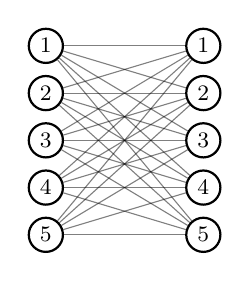
\begin{tikzpicture}
      \tikzstyle{every node} = [draw, circle, thick, inner sep = 2pt]
      \foreach \y in {0,...,4}{
        \pgfmathtruncatemacro{\yplusone}{5 - \y}
        \node(a\y) at (0,.6*\y) {\footnotesize\yplusone};
      }
      \foreach \y in {0,...,4}{
        \pgfmathtruncatemacro{\yplusone}{5 - \y}
        \node(\y) at (2,.6*\y) {\footnotesize\yplusone};
      }

      \foreach \x in {0,...,4}{
        \foreach \y in {0,...,4}{
          \path[opacity=0.5] (a\x) edge (\y);
        }
      }
    \end{tikzpicture}
  \end{center}
  \caption{Examples}
  \label{con_ex}
\end{figure}

\todo{\figref{con_ex}. It's just a placeholder right now}


Connectivity graphs also allow to graphically modelize how weights are tied in a neural layer. Let's suppose the $\Theta_ij$ are taking their values only into the finite set $K = \{w_1, w_2, \ldots, w_\kappa\}$ of size $\kappa$, which we will refer to as the \emph{kernel} of \emph{weights}. Then we can define a labelling of the edges $s: E \rightarrow K$. $s$ is called the \emph{weight sharing scheme} of the layer. This layer can then be formulated as $\displaystyle \forall v \in M, y_v = \sum_{u \in N, (u,v) \in E} w_{s(u,v)} x_u$. \figref{cnn} depicts the connectivity graph of a 1-d convolution layer and its weight sharing scheme.

\begin{figure}[h]
  \begin{center}
    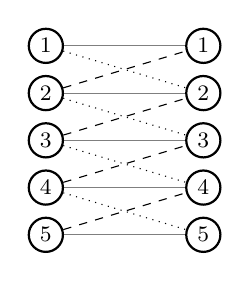
\begin{tikzpicture}
      \tikzstyle{every node} = [draw, circle, thick, inner sep = 2pt]
      \foreach \y in {0,...,4}{
        \pgfmathtruncatemacro{\yplusone}{5 - \y}
        \node(a\y) at (0,.6*\y) {\footnotesize\yplusone};
      }
      \foreach \y in {0,...,4}{
        \pgfmathtruncatemacro{\yplusone}{5 - \y}
        \node(\y) at (2,.6*\y) {\footnotesize\yplusone};
      }
      \path[opacity=0.5]
      (a0) edge (0);
      \path[dashed]
      (a0) edge (1);
      \path[dotted]
      (a1) edge (0);
      \path[opacity=0.5]
      (a1) edge (1);
      \path[dashed]
      (a1) edge (2);
      \path[dotted]
      (a2) edge (1);
      \path[opacity=0.5]
      (a2) edge (2);
      \path[dashed]
      (a2) edge (3);
      \path[dotted]
      (a3) edge (2);
      \path[opacity=0.5]
      (a3) edge (3);
      \path[dashed]
      (a3) edge (4);
      \path[dotted]
      (a4) edge (3);
      \path[opacity=0.5]
      (a4) edge (4);
    \end{tikzpicture}
  \end{center}
  \caption{Depiction of a 1D-convolutional layer and its weight sharing scheme.}
  \label{cnn}
\end{figure}


\todo{Add weight sharing scheme in \figref{cnn}}

\subsection{Computation graph}
\label{comp_graph}

\subsection{Underlying graph structure}
\label{inductive_graph}

\subsection{Graph-structured dataset}
\label{transductive_graph}

transductive vs inductive

\section{Special classes of graphs}

\subsection{Grid graphs}

\subsection{Spatial graphs}

\subsection{Projections of spatial graphs}

\newpage

\section{Subject disambiguation}

\section{Convolutions on graphs (draft)}

Defining a convolution on graphs is a challenging problem. Obviously, the underlying structure determined by a graph is not necessarily isomorphic to a set onto which the convolution is already defined. 

Related works: moura, spectral convolution with laplacian.

A convolution may comprise the following properties: bilinear, equivariant with respect to a certain class of isomorphism.

We shall first study classes of graphs onto which the convolution can be naturally defined before generalizing.

*Convolution without the edges

*Convolution on grids

*Convolution on lattice-regular graphs

*Convolution on product graphs

*Convolution on linear combination of circulant graphs

\subsection{Convolution without the edges}

We first consider a grid graph $\gve$ agnostically of its edges \ie $G \cong \bbz^2$. By restriction to compactly supported signals, this case encompass the case of images.

\begin{definition}\textbf{Transformation}\\
A \emph{transformation} $f: V \rightarrow V$ is a function with same domain and codomain. The set of transformations is denoted $\Phi(V)$. The set of bijective transformations is denoted $\Phi^*(V) \subset \Phi(V)$.

In case $f \in \Phi^*(V)$, it can act on $\cs(V)$ through the linear operator $L_f \in \cl(\cs(V))$ defined as:
\begin{gather*}
\forall s \in \cs(V), \forall v \in V, f(s)[v] := L_f s[v] = s[f^{-1}(v)]
\end{gather*}
\ie an entry of a transformed signal is obtained by doing a lookup of the entry of the original signal.

In case $f \notin \Phi^*(V)$, we can still define $L_f \in \cl(\cs(V))$, however we need to linearly aggregate the entries on the fibers:
\begin{gather*}
\forall s \in \cs(V), \forall v \in V, f(s)[v] := L_f s[v] = \agg\{s[u], u \in f^{-1}\{v\}\}
\end{gather*}
where $\agg$ can be for example the sum, the average, or the max, and $\agg(\emptyset) = 0$.
\end{definition}

\begin{definition}\textbf{Translation on $\cs(\bbz^2)$}\\
A translation on $\bbz^2$ is defined as a transformation $t \in \Phi^*(\bbz^2)$ such that
\begin{gather*}
\exists (a,b) \in \bbz^2, \forall (x,y) \in \bbz^2, t(x,y) = (x+a,y+b)
\end{gather*}
It also acts on $\cs(\bbz^2)$ with the notation $t_{a,b}$ \ie
\begin{gather*}
\forall s \in \cs(\bbz^2), \forall (x,y) \in \bbz^2, t_{a,b}(s)[x,y] = s[x-a, y-b]
\end{gather*}
For any set $E$, we denote by $\ct(E)$ its translations.
\end{definition}

The next proposition can be seen as a discretization of a classic result in distribution theory.

\begin{proposition}\textbf{Characterization of convolution operators on $\cs(\bbz^2)$}\\
On real-valued signals over $\bbz^2$, the class of linear transformations that are equivariant to translations is exactly the class of convolutive operations \ie
\begin{gather*}
\begin{cases}
 f \in \cl(\cs(\bbz^2))\\
 \forall t \in \ct(\cs(\bbz^2)), f \circ t = t \circ f
\end{cases}
 \Leftrightarrow \exists w \in \cs(\bbz^2), f = . \ast w
\end{gather*}
\label{prop:equi}
\end{proposition}

\begin{proof}
The converse is a direct consequence of the definitions:
\begin{align}
\forall s \in \cs(\bbz^2), \forall (a,b) \in \bbz^2, & \forall (\alpha, \beta) \in \bbz^2, \forall s' \in \cs(\bbz^2),\nonumber\\
 f_w(s)[a,b] & = \displaystyle \sum_i \sum_j s[i,j] \h{2} w[a-i, b-j] \tag{definition}\\
 f_w(\alpha s + \beta s')[a,b] & = \displaystyle \sum_i \sum_j (\alpha s + \beta s')[i,j] \h{2} w[a-i, b-j]\nonumber\\
 & = \alpha f_w(s)[a,b] + \beta f_w(s')[a,b] \tag{linearity}\\
f_w \circ t_{\alpha,\beta} (s)[a,b] & = \displaystyle \sum_i \sum_j t_{\alpha,\beta}(s)[i,j] \h{2} w[a-i, b-j]\nonumber\\
 & = \displaystyle \sum_i \sum_j s[i - \alpha,j - \beta] \h{2} w[a-i, b-j]\nonumber\\
 & = \displaystyle \sum_{i'} \sum_{j'} s[i',j'] \h{2} w[a - i' - \alpha, b - j'- \beta]\label{eq:bij}\\
 & = f_w (s)[a - \alpha,b - \beta]\nonumber\\
 & = t_{\alpha,\beta} \circ f_w (s)[a,b] \tag{equivariance}
\end{align}
Now let's prove the direct sense.
Let $f \in \cl(\cs(\bbz^2))$, $s \in \cs(\bbz^2)$. We suppose that $f$ commutes with translations.

For $(x,y) \in \bbz^2$ we denote by $\delta_{x,y}$ the dirac signal
\begin{gather*}
\delta_{x,y}[i,j] = \begin{cases} 1 & \text{if } (x,y) = (i,j)\\ 0 & \text{otherwise} \end{cases}
\end{gather*}
Then,
\begin{gather*}
s = \displaystyle \sum_i \sum_j s[i,j] \h{2} \delta_{i,j}
\end{gather*}
By linearity of $f$ and then equivariance to translations:
\begin{align*}
f(s) & = \displaystyle \sum_i \sum_j s[i,j] \h{2} f(\delta_{i,j})\\
 & = \displaystyle \sum_i \sum_j s[i,j] \h{2} f \circ t_{i,j} (\delta_{0,0})\\
 & = \displaystyle \sum_i \sum_j s[i,j] \h{2} t_{i,j} \circ f (\delta_{0,0})
\end{align*}
By denoting $w = f (\delta_{0,0}) \in \cs(\bbz^2)$, we obtain:
\begin{align}
\forall (a,b) \in \bbz^2, f(s)[a,b] & = \displaystyle \sum_i \sum_j s[i,j] \h{2} t_{i,j}(w)[a,b] \label{eq:conv}\\
 & = \displaystyle \sum_i \sum_j s[i,j] \h{2} w[a-i, b-j] \nonumber\\
\text{\ie } f(s) & = s \ast w \nonumber
\end{align}
\end{proof}

\begin{remark}\textbf{Superiority of CNNs over MLPs}\\
In deep learning, an important argument in favor of CNNs is that convolutional layers are equivariant to translations. Intuitively, that means that an object in an image should produce the same features independently of its position in the image. In fact, as a consequence of~\propref{prop:equi} any neural layer that is equivariant to translations is also a convolutional layer. So every equivariant functions are in the search space of each layers of CNNs. When such property is known to hold for the objective function, then the reduction of parameters from an MLP to a CNN is done with strictly no loss of effective expressivity. On the contrary, it helps the training to search in a much more confined space.
\end{remark}

\begin{remark}\textbf{Construction of convolutions}\\
As \propref{prop:equi} is a complete characterization of convolutions, it can be used to define them. This can be a lead to define convolutions on graphs, either by defining meaningful translations on graphs (see \secref{}), or by a construction that would be equivariant to a certain class of transformations. For the later possibility, we see in the proof of \propref{prop:equi} that the reindexing of \eqref{eq:bij} requires bijective transformations
\end{remark}


It shall then be natural that convolutions are constructed from this characterization.

To construct convolution operators on any graph $G$ with this characterization, we note from the former proof that all we need is the definition of the translations $t_{i,j}$, which have no reason whatsoever to be defined naturally on~$G$. More generally, any class of transformations on the vertices that would be entirely determined by their image on a certain vertex would be enough to construct a class of convolution operators. Such transformations would replace the translations $t_{i,j}$ in the construction of a convolution operator in line \eqref{eq:conv} of the previous proof. This give rize to the following definitions.

\begin{definition}\textbf{Grounded set of transformations}\\
A set of transformations over a graph $\gve$, \emph{grounded} on a vertex $v_0 \in V$, denoted $\cp_{v_0} \subset \Phi(V)$, is a set that is in one-to-one correspondence with $V$, such that $\forall v \in V, \exists! p_v \in \cp_{v_0}, p_v(v_0) = v$.
\end{definition}

We have $\cp_{v_0} = \order(G) \in \bbn \cup \{+\infty\}$. For notational convenience we drop the subscript $_{v_0}$ in what follows.

\begin{definition}\textbf{$\cp$-equivariant convolution operator}\\
Let $\gve$ a graph, not necessarily a grid. Let $\cp$ a grounded set of transformations. Then, the  $\cp$-equivariant convolution operator $f_w$ is defined as
\begin{gather*}
\forall s \in \cs(V), f_w(s) = s \ast_{\cp} w = \displaystyle \sum_v s[v] \h{2} p_v(w)
\end{gather*}
\end{definition}

\begin{claim}\textbf{Characterization of $\cp$-eq. convolution operator}\\
The class of linear graph signal transformations that are equivariant to a grounded set $\cp$ is exactly the class of $\cp$-equivariant convolutive operations.
\end{claim}

\begin{proof}
By construction of $\cp$-equivariant convolutions, the proof is similar to the one of \propref{prop:equi}.
\end{proof}



*note on drawbacks. If transformations were a group -> group convolution.
*note on morphisms

\subsection{Special classes of graphs}

% \begin{definition}\textbf{Infinite graph}\\
% An \emph{infinite graph} is defined by natural extension of the notion of graph $G=\langle V,E \rangle$ where $V$ and $E$ can be infinite. We denote $\order{G} = \infty$.
% \end{definition}

\begin{definition}\textbf{Graph automorphisms}\\
A graph automorphism of a graph $\gve$ is a bijection in the vertex domain $\phi: V \rightarrow V$ such that $\{u,v\} \in E \Leftrightarrow \{\phi(u), \phi(v)\} \in E$. We denote $\ca(G)$ the group of automorphism on $G$.

We denote by $\ce(\phi)$ the set of input-output mapping of $\phi$, defined as $\ce(\phi) = \{ (x,y) \in V^2, \phi(x) = y \}$.

A graph automorphism $\phi$ is said to be \emph{edge-constrained} (EC) if $\ce(\phi) \subseteq E$. We denote $\ca_{\EC}(G)$ the set of edge-constrained automorphism on $G$.
\end{definition}

\begin{definition}\textbf{Orthogonality}\\
Two graph automorphisms $\phi_1$ and $\phi_2$ are said to be orthogonal, if and only if $\ce(\phi_1) \cap \ce(\phi_2) = \emptyset$, denoted $\phi_1 \bot \phi_2$. They are said to be aligned otherwise.

Similarly, we define orthogonality of $r$ automophisms as $\phi_1 \bot \cdots \bot \phi_r \Leftrightarrow \ce(\phi_1) \cap \cdots \cap \ce(\phi_r) = \emptyset$
\end{definition}


\subsection{Lattice-regular graph}


\begin{definition}\textbf{Lattice-regular graph}\\
A lattice-regular graph is a regular graph that admits $r$ orthogonal edge-constrained automorphisms, where $r$ is its degree.
\end{definition}


%\subsubsection{Grids}

%\subsubsection{Lattices}

%\subsubsection{Spatial graphs}

%\subsubsection{Projections of spatial graphs}
\newpage